\chapter{ILOCI: ROBUST GENOME ANNOTATION AND ANALYSIS FOR PROVISIONAL GENOME ASSEMBLIES}

A paper to be submitted to \textit{Genome Biology}.

\noindent\hfil\rule{0.5\textwidth}{.4pt}\hfil

Standage DS, Brendel VP

\section{Abstract}

\noindent \textbf{Background:}
The rate at which new draft genome sequences and corresponding annotations are being produced outpaces the scientific community's capacity to refine these drafts into ``finished" reference-quality data resources.
Scientists must be able to evaluate newly sequenced genomes in the context of previously published data, requiring summaries of genome content that can be quickly computed and meaningfully compared without the support of a large model organism research community.
As annotation quality will necessarily vary within and across data sets, the ability to select subsets of only those data that are well supported is critical for distinguishing technical artifacts from biological effects.

\noindent \textbf{Results:}
We introduce a new framework for genome analyses based on parsing an annotated genome assembly into distinct \textit{interval loci (iLoci)}.
We demonstrate that iLoci provide an alternative coordinate system that is robust to changes in assemblies and annotations, and facilitates granular quality control of genome data.
We discuss how statistics computed on iLoci reflect various characteristics of genome content and organization, and illustrate how this can be used to establish a baseline context for evaluating a new genome assembly and annotation.
We also introduce a well-defined measure of relative genome compactness, and more generally show how iLoci reveal the extent of gene clustering genome wide.

\noindent \textbf{Conclusions:}
The iLocus framework, available as open source software as part of the AEGeAn Toolkit (\url{https://brendelgroup.github.io/AEGeAn}), provides a comprehensive solution to common challenges in annotation and analysis of non-model genomes.

\section{Background}

The ready availability of Next-Generation Sequencing (NGS) technologies has resulted in genome data for thousands of species, with no slowing down of data accumulation in sight.
Given this volume of data, fast and accurate computational approaches are needed now more than ever to process the initial sequence data into meaningful units of knowledge about the sequenced genome.
The conventional paradigm for that task from a few years ago is outdated.
At that time one could expect community groups to carefully assemble and annotate the genomes of their expertise, resulting over a period of time in gap-filled assemblies and refined documentation of genome content in terms of protein-coding genes, non-coding RNA genes, transposable elements, repetitive sequences, and so forth.
Such time-consuming and expensive efforts are impractical for the organisms currently being sequenced with NGS technologies.

Out of necessity, the old paradigm has for the most part been replaced by an implicit new standard:  genome data are presented as massive short read  collections available from databases like the NCBI Sequence Read Archive \cite{SRA} and in processed form as sets of assembled and computationally annotated scaffolds.
Concomitantly, downstream analyses of these data have to be adjusted to  scope and quality limitations intrinsic to the new data production process.
First, assembly completeness will vary depending on the degree of read coverage and genome complexity (size and repetitiveness).
Typically, assemblies will consist of tens to hundreds of large scaffolds, which in the best case can be ordered into linkage groups that approach pseudo-chromosomes; and in addition, manifold more short scaffolds, typically unplaced relative to any linkage groups.
Second, annotation will commonly not have been expertly curated, but rather have resulted from first-pass outputs of annotation workflows such as AUGUSTUS \cite{AUGUSTUS}, MAKER-P \cite{MAKERP}, BRAKER1 \cite{BRAKER1}, or NCBI Gnomon \cite{Gnomon}.

Another challenge can be the more temporary nature of the data.
As additional sequences can often be acquired cheaply and easily for a species (for example, genomic DNA reads for libraries of different insert sizes; RNA-Seq reads from transcriptome studies under various conditions; or spliced alignments of protein sequences from a newly annotated, closely related species), both the species' genome assembly and its genome annotation may change.
However, in the common scenario laid out above, the additional analyses will typically come without the community support to carefully sort out and document all the changes.
Thus, over a short span of several years, there may be several annotation versions even for a single stable genome assembly, and it becomes difficult to track references to particular genes and genome features.
A pertinent example from our experience is provided by the number of concurrent annotations in recent use for the honey bee (\textit{Apis mellifera}) genome \cite{OGS1.0, OGS3.2, NCBIAm102}.

How then should one compare results of a study on a current genome assembly and annotation version with previous results in the literature that used a prior
assembly/annotation pair?
How could one derive subsets of just those gene models that are solidly supported by evidence, to the extent that future genome-wide assembly/annotation improvements will not invalidate these current models?
How does one disentangle artifacts of incomplete or inaccurate assembly/annotation from genuine species-specific genome features?

A solution to the problem must address both reproducibility of analyses on genome data and scalability to accommodate thousands of genomes, each potentially with multiple assemblies and annotations.
At the core of a solution must be the ability to distinguish what has changed and what has remained invariant from one assembly/annotation pair to another.
Discriminating between solid, reliable annotations and annotations of uncertain quality is also crucial in order to enable separation of technical artifacts from effects of interest rooted in the underlying genome biology.
Typical examples of this challenge include  annotation of UTRs, ncRNA genes, or identification of transposable elements: comparing two genome annotations, one would like to know whether differences in UTR lengths or ncRNA gene and transposon content are due to insufficient data for annotation, annotation workflow settings, or genome evolution.

The ParsEval software \cite{StandageBrendel2012} provides a convenient tool for comparing two sets of annotations for the same genome assembly.
Here we introduce a more general concept and associated software applicable to both single genome analyses and comparisons across assemblies, annotations, and genomes.
The basic idea is to represent a given assembly/annotation pair as a set of distinct units that can be largely independently characterized and updated.
We show how the parsing of a genome into such distinct \textit{iLoci} provides a suitable ``coordinate system" for working with rapidly changing genome assembly/annotation data.
Applications to genome project data for various plant and animal species demonstrate how \textit{iLoci} analyses can give insights into genome organization and features, as well as assembly and annotation status.

\section{Methods}

\subsection{Toolkit design}
Motivated by the challenges of present day genome data reviewed in the \textbf{Background} section, we have developed a toolkit for the \textbf{A}nalysis and \textbf{E}valuation of \textbf{Ge}nome \textbf{An}notations (\textbf{AEGeAn} \cite{AEGeAn}).
The design of the toolkit followed general principles to achieve reproducible and scalable applications that are easy to use, available as open source code, and integrated with existing tools such as GenomeTools \cite{GenomeTools, GenomeToolsWebsite}.
From a user perspective, the toolkit is meant to work with well-defined inputs consisting of one or more genome sequences paired with associated genome annotation, provided in multi-FASTA and GFF3 \cite{GFF3} formats, respectively.
As discussed in the \textbf{Background} section, an input pair can represent a mature model organism genome/annotation version or an incomplete assembly with preliminary annotation.
Either way, the toolkit will allow the user to probe genome assembly content and organization, with results reflecting both underlying genome features and the degree of assembly/annotation completeness and accuracy.
We show how comparison of different data sets suggests interpretation of results that distinguishes the two possibilities.

The current implementation of the AEGeAn Toolkit provides summary statistics covering a large range of specific questions concerning genome content and organization as well as utility functions to select subsets of genome features for further analysis.
Before discussing algorithmic and programming details, we list a number of specific questions that AEGeAn tools address.
The \textbf{Results} section demonstrates the usefulness of the tool in practical applications.

A first range of questions addresses genome content:
How many genes are annotated for a particular assembly/annotation pair?
What proportion of the genome is occupied by these genes?
What can be said about their length, number of exons, nucleotide composition, and other characteristics?
What fraction of genes are protein-coding versus non-coding RNA genes?
How many of the gene models have support from transcript evidence, and how many genes can be identified as likely homologs of genes in other species?
As we will illustrate later, these seemingly simple questions actually require very precise processing of the annotation file to be reproducibly and meaningfully answered.
In particular, the handling of alternative transcription as well as overlapping gene models needs to be unambiguously defined.
The AEGeAn Toolkit includes functions that subselect gene loci based on user-defined characteristics.
These functions facilitate the generation of reliable data sets for applications such as codon usage statistics, training of gene prediction models, or identification of transcription regulatory motifs.

A second range of questions addresses genome organization:
How densely or sparsely packed are the genes?
Is there clustering of genes, and if so, how large are these clusters and what types of genes occur in clusters?
More generally, how is the intergenic space organized?

Lastly, all of the above questions are of interest in a comparative genomics context.
To what extent are genomes within a clade of species similarly organized?
And, maybe even more intriguingly, to what extent is genome organization functionally important?


\subsection{Conceptual definition of interval loci}
To address the toolkit design prescriptions, we introduce a precise parsing of an assembly/annotation pair into smaller units, termed \textit{interval loci}, that provide a robust, granular, and dynamic data set for answering the biological questions posed above.
Each interval locus (or \textit{iLocus}) is intended to capture the local genomic context of a genic or intergenic space, providing an alternative coordinate system to the conventional scaffold-based system that is robust to changes in assemblies and annotations.
Conceptually, an iLocus is a genomic interval, the boundaries of which are computed from annotated gene models, with an extension to include probable adjacent \textit{cis}-regulatory regions.
The precise procedure for computing iLoci is described in detail in the next section.

iLoci can be distinguished by various characteristics, as summarized in \textbf{Figure \ref{Fig:iLocusDesignations}}.
iLoci containing genes are referred to as \textit{giLoci}, with those encoding protein-coding genes labeled as \textit{piLoci} and those containing non-coding genes labeled as \textit{niLoci}.
piLoci harboring multiple overlapping gene models are designated complex (\textit{ciLoci}), while those with a single isolated gene model are designated simple (\textit{siLoci}).
iLoci containing no gene models are designated as intergenic (\textit{iiLoci}) if they are flanked on both sides by genes, or as incomplete fragments (\textit{fiLoci}) if they are are flanked on either side by an end of the scaffold.

To illustrate these concepts, \textbf{Figure \ref{Fig:iLoci}} shows the parsing of a hypothetical scaffold into its constituent iLoci.
The parsing captures an intuitive and practical decomposition of the genome.
The piLoci comprise a superset of protein-coding genes when reporting gene number or calculating descriptive statistics on gene features.
However, more reliable results would be expected from the siLoci, or even better a subset of the siLoci with well supported gene models.
The ciLoci will typically require a whole lot more attention to establish whether the overlapping gene models reflect observed transcription or are artifacts of unresolved annotation conflicts.


\subsection{Operational definition of iLoci}
%\subsubsection*{Basic procedure}
Computing iLoci for an assembled contig/scaffold/pseudo-chromosome $S$ depends on a set of intervals $G$ (corresponding to gene models annotated on $S$) and an extension parameter $\delta$.
The basic procedure is described in \textbf{Algorithms \ref{Alg:ComputeiLoci}} and \textbf{\ref{Alg:ExtendIntervals}}.
In brief, the $\textsc{ComputeLoci}$ algorithm computes a new set of intervals $L$ such that any two overlapping elements $g_m, g_n \in G$ are bounded by the same interval $loc \in L$.
Although the algorithm is general, here $g_m$ and $g_n$ refer to gene bodies, defined as the interval from the start to the end of the respective annotated transcription events.
The $\textsc{ExtendIntervals}$ algorithm then assesses each pair of adjacent intervals $loc_m, loc_n \in L$ and determines how far the intervals can be extended toward each other and whether any additional space remains between them for the creation of a third interval:
if the number of nucleotides separating the two intervals $dist(loc_m, loc_n) > 3 \delta$ nucleotides, then $loc_m$ and $loc_n$ will be extended toward each other by $\delta$ nucleotides, each designated as a giLocus, and the remaining space between them will be designated as an iiLocus;
if $2\delta < dist(loc_m, loc_n) \leq 3\delta$, then $loc_m$ and $loc_n$ are extended toward each other equally until they meet, with extensions potentially as long as $1.5\delta$, to prevent annotating an extremely short iiLocus;
if $dist(loc_m, loc_n) \leq 2\delta$, $loc_m$ and $loc_n$ will each be extended by $\delta$ resulting in overlapping iLoci.
In the two latter cases the toolkit records a zero-length iLoci (\textit{ziLocus}) between the adjacent giLoci for consistency and calculation of cumulative statistics described below.

\begin{algorithm}
\caption{Compute giLocus boundaries}
\label{Alg:ComputeiLoci}
\begin{algorithmic}[1]
\Procedure{Overlap}{$\textit{loc}, G$}
\State $O \gets loc$
\For{$g' \in G$}
    \If{$g'$ overlaps with $\textit{loc}$}
        \State $O \gets O \cup g'$
        \State mark $g'$ as visited
    \EndIf
\EndFor \\
\Return $O$
\EndProcedure
\Procedure{ComputeLoci}{$G, \delta$}
\State $L \gets \emptyset$
\For{interval $g \in G$}
    \If{$g$ is marked as visited}
        \State \textbf{continue}
    \EndIf
    \State interval $\textit{loc} \gets g$
    \State mark $g$ as visited
    \While{$\textsc{Overlap}(\textit{loc}, G) \supset \textit{loc}$}
        \State $\textit{loc} \gets \textsc{Overlap}(\textit{loc}, G)$
    \EndWhile
    \State $L \gets L \cup \{\textit{loc}\}$
\EndFor
\State $\textsc{ExtendIntervals}(L, \delta)$ \\
\Return $L$
\EndProcedure
\end{algorithmic}
\end{algorithm}

\begin{algorithm}
\caption{Extend giLocus boundaries, identify iiLoci}
\label{Alg:ExtendIntervals}
\begin{algorithmic}[1]
\Procedure{ExtendIntervals}{$L, \delta$}
\For{adjacent intervals $x, y \in L$}
\If{$\textit{dist}(x, y) < 2\delta$}
    \State $\textit{End}(x) \gets \textit{End}(x) + \delta$
    \State $\textit{Start}(y) \gets \textit{Start}(y) - \delta$
\ElsIf{$2\delta < \textit{dist}(x, y) < 3\delta$}
    \State $\textit{midpoint} \gets \left\lfloor \textit{Average}\left(\textit{End}(x), \textit{Start}(y)\right) \right\rfloor$
    \State $\textit{End}(x) \gets \textit{midpoint}$
    \State $\textit{Start}(y) \gets \textit{midpoint} + 1$
\Else
    \State $\textit{End}(x) \gets \textit{End}(x) + \delta$
    \State $\textit{Start}(y) \gets \textit{Start}(y) - \delta$
    \State interval $iiLocus \gets [ \textit{End}(x)+\delta+1, \textit{Start}(y)-\delta-1 ]$
    \State $L \gets L \cup \{ iiLocus \}$
\EndIf
\EndFor
\EndProcedure
\end{algorithmic}
\end{algorithm}

%\subsubsection*{Post-processing to refine iLoci}
The iLocus parsing procedure is designed with the canonical case of gene organization in mind: a single gene model flanked on both sides by hundreds or thousands of nucleotides of intergenic space.
All eukaryotic genomes have exceptions to this case, some to a greater extent than others.
The basic parsing procedure can handle some exceptions, such as genes separated by very little intergenic space, but there are additional exceptions that occur frequently enough to merit additional post-processing and refinement.

The basic procedure places two gene models in the same iLocus if their gene bodies have any overlap.
While this is intended to capture gene models that may be conflicting or misannotated and in need of additional attention to resolve coordinates, an unintended consequence is the occasional grouping of genes with a trivial amount of incidental overlap.
For example, if two genes---each a few kilobases in length---happen to have 10-20 nucleotides of overlap in their UTRs, they should be separated and handled as distinct loci.
In post-processing, we enable splitting of such trivially overlapping iLoci by introducing two additional parameters: $\omega$, the number of nucleotides that two gene models must overlap to remain in the same iLocus, and $\kappa$ indicating whether that overlap is calculated using entire gene bodies ($\kappa = 0$) or just the coding sequences ($\kappa = 1$).

The initial procedure also groups non-coding RNA genes and protein-coding genes together if they overlap.
In post-processing, ncRNA genes and protein-coding genes are treated separately and will not be grouped in the same iLocus regardless of overlap, although overlapping ncRNA genes are grouped in the same niLocus.

An additional exception occurs when a gene resides completely within a single intron of another gene.
These genes are placed in the same iLocus during the initial parsing procedure, but can be separated into distinct iLoci during post-processing.


\subsection{Implementation}
In keeping with the conventions implemented by the GenomeTools library \cite{GenomeTools}, most of the core functionality of the AEGeAn Toolkit \cite{AEGeAn} is implemented by means of \textit{node streams} for sequential processing of genome features that are represented as \textit{feature graphs}.
In brief, genome features such as genes, exons, UTRs, and coding sequences are represented as nodes in a directed acyclic graph, and parent/child relationships between features, denoted by \textit{ID} and \textit{Parent} attributes in GFF3, are represented as edges in the graph.
Each connected component (CC) in the graph, typically corresponding to a gene and its subfeatures, is then processed sequentially by one or more node streams, each designed for a specific annotation processing task.
One advantage of this approach is its low memory footprint, as at most only a small number of CCs need be loaded into memory at any given moment.

The \textit{AgnLocusStream} module in the AEGeAn Toolkit implements a node stream for computing iLocus boundaries.
This node stream expects as input gene annotations (CCs with a gene feature as the root node) sorted by genomic position, but it is designed to work with arbitrary feature types.
Initially, the node stream will collect a single gene feature from the input and store it in a buffer.
Then, as subsequent gene features are collected, they are tested for overlap with the current iLocus (buffer) and accumulated as long as their leftmost position is less than or equal to the rightmost position of the buffer.
When the node stream encounters a gene feature that does not overlap with the buffer, a giLocus feature is created, all the genes in the buffer are assigned as children to the giLocus, a reference to the giLocus is stored temporarily in the node stream, and the giLocus is emitted for further processing or storage.
Later, as the subsequent giLocus is emitted, the adjacent pair of giLoci are extended toward each other and, when appropriate, an iiLocus is created and emitted, as described in \textbf{Algorithm \ref{Alg:ExtendIntervals}}.

The AEGeAn Toolkit's \textit{AgnLocusRefineStream} module implements a node stream for post-processing the initial iLocus designations, as described in the previous section.
Any genes belonging to the same giLocus that do not overlap by at least $\omega$ nucleotides in their gene bodies (or coding sequences if $\kappa = 1$), as well as genes contained completely within the intron of another gene, are split into distinct overlapping giLoci.

The \textit{LocusPocus} program is a command-line tool included in the AEGeAn Toolkit distribution which provides a user interface to the \textit{AgnLocusStream} and \textit{AgnLocusRefineStream} modules.
A detailed description of command-line usage and program inputs and outputs is provided in the \textbf{Supplementary Methods}.

\subsection{Genome content statistics}
As discussed in the \textbf{Background} section, describing genome characteristics and comparing across species requires selection of reliable subsets of data for analysis.
The precise selection criteria used will depend on the questions being asked, but commonly involve a small set of descriptive statistics that can easily be computed from the iLocus sequence and/or associated annotation.
These include the length and nucleotide composition of the iLocus itself, as well as the count, length, and composition of corresponding features such as genes, RNAs, exons, introns, and coding sequences.
Statistics are computed by invoking the \textit{stats} task of the \textit{genhub-build.py} script (see \textbf{Supplementary Methods}) and are stored in tab-separated plain text (.tsv) files to facilitate importing into popular statistical computing packages.

Additional characteristics, such as the quality and homology status of gene models, are not always readily accessible from the iLocus sequence or annotation but can be computed and attached to an iLocus annotation using key-value pairs in GFF3's \textbf{attribute} column.
Annotation quality can be measured with statistics such as Maker's \textit{annotation edit distance} \cite{AED} or the GAEVAL \textit{integrity score} \cite{GAEVAL}, and  homology status can be determined via BLAST search or clustering of iLocus protein products.
Attaching these characteristics to the iLocus provides additional features on which to filter data.

Descriptive statistics are reported only for a single annotated transcript at each iLocus to ensure aggregate statistics are not biased by redundancy in the data from, for example, genes with many annotated isoforms.
The reported transcript is selected according to the amino acid length of its translation product: the transcript with the longest product is reported.
In cases where multiple transcripts have translation products of identical length, the transcript with the lexicographically smallest \textbf{ID} attribute is reported, ensuring reproducible and deterministic reporting.

Cumulative lengths of different iLocus types are calculated after proper accounting of any iLocus overlaps to ensure each nucleotide in the genome is counted only once (see \textbf{Supplementary Methods}).
When reported as a fraction of the entire genome, the genomic space occupied for different iLocus categories is calculated as a fraction of \textit{effective genome size}---the total number of nucleotides in the genome that do not reside within fiLoci---to mitigate potentially confounding inflation of genome size by many short unannotated sequences or sequence fragments.

\subsection{Genome organization statistics}
Beyond genome content, the iLocus framework also allows to systematically study different aspects of genome organization.
Here we focus on gene orientation and spacing: are there species-specific patterns of gene arrangements, and how do natural genomes differ in these respects from statistical expectation?
Because of the flexible design of the code base described in the \textbf{Implementation} section, these questions can easily be generalized and extended, for example with respect to selection of subtypes of genic loci.

To study gene orientation, the \textit{LocusPocus} program reports for each iiLocus the orientation of the flanking giLoci as FF (forward $>>$), RR (reverse $<<$), RF (outward $<>$), or FR (inward $><$).
In the case that an iiLocus is flanked by one or more ciLoci, the orientation of the gene models directly flanking the intergenic space are reported.
These data are used to identify the longest stretches of genes all on the forward strand, all on the reverse strand, or periodically alternating between strands.
Differences in occurrence numbers and lengths of outward and inward iiLoci are also determined for possible interpretation in terms of promoter architecture.

Long iiLoci are flagged as regions for annotation review.
More generally, for each giLocus the lengths of the flanking iiLoci are reported.
In cases where a giLocus abuts or overlaps with another giLocus, the corresponding iiLocus length is set to zero, and the number of overlapping nucleotides is recorded.
The software tracks these cases as \textit{zero-length iiLoci} (\textit{ziLoci}).
The iiLoci lengths are used in two different ways to reveal gene spacing characteristics.
The distribution of aggregate lengths of $n$ adjacent iiLoci shows the mode of typical gene spacings as well as outliers.
%Should we use the percentage of genes in the genome that are flanked on both sides by intergenic space, those that have intergenic space only on one flank, and those flanked tightly on both sides by other genes.
Secondly, overlapping or abutting giLoci are collapsed into \textit{merged iLoci} (\textit{miLoci}) during post-processing and represent gene clusters.
Our results show that relative counts and lengths of miLoci compared to non-merged siLoci provide robust measures of genome compactness.

To evaluate observed gene spacing patterns with statistical expectation, we implemented a procedure to generate randomized gene arrangements relative to the input genome annotation in GFF3 format.
First, iLoci are computed with $\delta=0$ to identify the precise boundaries of annotated genic regions.
Next, giLoci are removed from the sequence and the remaining iiLoci are concatenated.
Then, new positions are randomly selected from a uniform distribution for re-inserting the giLoci in shuffled order into the sequence.
As each giLocus is re-inserted, the genomic sequence is expanded, and all downstream re-insertion sites are adjusted accordingly.
Re-running the iLocus parsing procedure and computing neighbor statistics on these random arrangements provides a baseline for comparison, revealing how genome annotations as observed differ (at the genome scale) from what could be expected from a completely random arrangement of genes.


\subsection{Comparing assembly/annotation pairs: iLocus stability}
Given two assembly/annotation versions for the same genome, we evaluate the stability of iLoci across the two versions using sequence alignment and interval overlap.
Specifically, iLocus sequences from the earlier assembly/annotation version (version \textit{A}) are aligned to the genome of the newer version (version \textit{B}), and the interval of each alignment is compared to the intervals of iLoci annotated on \textit{B}.
An iLocus from \textit{A} is designated stable if the following criteria are satisfied: it aligns to genome \textit{B} with at least 95\% identity; an iLocus from \textit{B} overlaps with at least 90\% of the aligned iLocus sequence from \textit{A}; and the alignment interval overlaps with at least 90\% of that same iLocus from \textit{B}.

For this study, we used Vmatch \cite{Vmatch} to compute iLocus alignments (using options \texttt{-complete -e 5b -identity 95 -d -p -showdesc 0}).
As a preliminary step, we used RepeatMasker \cite{RepeatMasker,RepBase} and bedtools \cite{bedtools} to identify and filter out iLoci with substantial repetitive content to make alignment computations tractable.
Specifically, any iLocus with at least 500 bp or 25\% repetitive content was excluded from the Vmatch alignment procedure.


\subsection{Comparing genome content and organization between related genomes: homologous iLoci}
Given a set of annotated genome assemblies for a clade of related species, we compute \textit{homologous iLoci (hiLoci)} via a protein clustering procedure.
For each species, a representative protein sequence is selected for each piLocus (as described in the \textbf{Genome content statistics} section).
The distinct protein complements from all species are then combined, and the aggregate collection of protein sequences is clustered using cd-hit \cite{cdhit}.

In brief, cd-hit processes proteins iteratively from longest to shortest.
The first protein is assigned to a cluster by itself and is designated the \textit{representative sequence} of the cluster.
Each subsequent protein is compared to all previous clusters:
if the alignment of the protein to a cluster's representative sequence satisfies the specified sequence identity, length similarity, and alignment coverage criteria, it is added to that cluster, and the program advances to the next protein;
if a protein cannot be added to any cluster by user-specified clustering criteria, it is placed in a new cluster by itself and designated the representative sequence of that cluster.

Following the clustering procedure, a \textit{homologous iLocus (hiLocus)} is designated for each protein cluster and the piLoci corresponding to the proteins in that cluster are assigned to that hiLocus.
The hiLocus thus provides a link between piLoci from related species and a relative measure of how well conserved the corresponding protein is within the given clade.

This protein clustering procedure is invoked using the \textit{cluster} task of the \textit{genhub-build.py} script.
The script provides the following default clustering criteria, although these defaults can be overridden and additional criteria set by the user.
The default parameters are as follows: sequence identity $\geq$ 50\%; length difference $\leq$ 65\%; alignment coverage for longer sequence $\geq$ 75\%; alignment coverage for shorter sequence $\geq$ 85\%.
On the command line these parameters are specified as \texttt{-c 0.50 -s 0.65 -aL 0.75 -aS 0.85}.


\subsection{Data sets analyzed}
To demonstrate the utility of iLoci for providing a descriptive overview of genome composition and organization, we retrieved RefSeq genome assemblies and corresponding annotations for ten model organisms (complete species names listed shown \textbf{Table \ref{Table:iLocusCountsModOrg}}).
Species were selected to provide a broad sampling of eukaryotic diversity, with a preference for robust model organisms with mature chromosome-level genome assemblies and extensive community-supported annotation.
For each species, we computed iLoci and associated feature statistics, including length, nucleotide composition, exon count, and \textit{effective length} using standard GenHub build tasks as described before.
Precise configurations and commands run are described in detail in the \textbf{genome-summary} section at \url{https://github.com/BrendelGroup/IntervalLoci}.

Using iLocus summaries of these ten model organisms as a baseline for comparison, we characterized the genome content and organization of three additional species of interest that serve as important experimental models for evolutionary and ecological studies.
The alga \textit{Volvox carteri} is the focus of research on the evolution of cellular complexity and development, and was the second alga (after \textit{Chlamydomonas reinhardtii}) to have its genome sequenced.
The paper wasp \textit{Polistes dominula} is an important model for studying the evolution of social behavior, and provided one of the first sequenced genomes of a vespid wasp \cite{PdomGenome}.
The water flea \textit{Daphnia pulex} is a species of ecological and evolutionary interest, and was the first crustacean to have its genome sequenced \cite{DaphniaGenome}.
Genomes for these three species were processed using the same procedure as the ten model organisms (see \url{https://github.com/BrendelGroup/IntervalLoci}).


%\subsubsection*{Classifying hiLoci from a clade of 9 chlorophyte species}
To investigate the extent of gene conservation in the green algae (phylum: Chlorophyta), we collected and processed data for nine chlorophyte species (\textit{Auxenochlorella protothecoides}, \textit{Chlamydomonas reinhardtii}, \textit{Chlorella variabilis}, \textit{Coccomyxa subellipsoidea}, \textit{Micromonas pusilla}, \textit{Micromonas sp. RCC299}, \textit{Ostreococcus lucimarinus}, \textit{Ostreococcus tauri}, and \textit{Volvox carteri}), as well as four land plants (\textit{Arabidopsis thaliana}, \textit{Brachypodium distachyon}, \textit{Medicago truncatula}, and \textit{Oryza sativa}) as an outgroup.
Retrieval of annotations and sequences and calculation of hiLoci was invoked using standard procedures as described before (see \mbox{\textbf{chlorophyta}} section at \url{https://github.com/BrendelGroup/IntervalLoci}).
Following the protein clustering procedure, each hiLocus was assigned a preliminary classification: \textit{highly conserved} if it had a representative from each of the nine chlorophyte genomes; \textit{conserved} if it had a representative from at least four chlorophyte genomes; \textit{matched} if it had a representative from at least two genomes (including the outgroups); and \textit{unmatched} if it had a representative from only a single genome.

iLoci initially classified as \textit{unmatched} were subjected to additional screening to distinguish conserved proteins lacking a nearly-full-length match (due to incomplete or incorrect annotation, or true evolutionary divergence) from orphan proteins without any reliable match.
iLoci with a BLASTP match against another species (\texttt{-evalue 1e-10}) were reclassified as \textit{matched}, while those lacking a match were reclassified as \textit{orphan}.










\section{Results}

\subsection{iLoci provide an informative decomposition of genome content}

\begin{table}[t]
\caption{iLocus content of genomes from ten model organisms and three additional species.}
\label{Table:iLocusCountsModOrg}
\begin{tabularx}{\textwidth}{lrrrrrrrr}
\hline
                            Species &  Mb\textsuperscript{1} &  \#Seq\textsuperscript{2} &       fiLoci &       iiLoci &       niLoci &       siLoci &       ciLoci   \\ \hline
\textit{Saccharomyces cerevisiae}   &                   12.1 &                        16 &           11 &          289 &          393 &        5,704 &           90   \\
\textit{Caenorhabditis elegans}     &                  100.3 &                         6 &            4 &        7,783 &       19,230 &       20,071 &           81   \\
\textit{Chlamydomonas reinhardtii}  &                  120.2 &                     1,556 &        1,487 &        6,248 &            0 &       14,254 &           42   \\
\textit{Medicago truncatula}        &                  412.8 &                     2,186 &        2,325 &       36,465 &        1,075 &       50,444 &            0   \\
\textit{Anopheles gambiae}          &                  265.0 &                     8,089 &        8,041 &        7,724 &          639 &       12,184 &          120   \\
\textit{Drosophila melanogaster}    &                  143.7 &                     1,869 &        1,849 &        3,436 &        3,289 &       13,115 &          239   \\
\textit{Xenopus tropicalis}         &                 1437.5 &                     7,727 &        8,004 &       18,580 &        5,199 &       21,704 &          135   \\
\textit{Danio rerio}                &                 1371.7 &                     1,060 &        1,276 &       23,978 &       12,776 &       26,229 &          166   \\
\textit{Mus musculus}               &                 2725.5 &                        21 &           42 &       23,689 &       14,103 &       21,305 &          218   \\
\textit{Homo sapiens}               &                 3088.3 &                        24 &           48 &       22,242 &       16,995 &       19,067 &          399   \\ \hline
\textit{Volvox carteri}             &                  137.7 &                     1,251 &        1,198 &        7,790 &            0 &       14,346 &           44   \\
\textit{Polistes dominula}          &                  208.0 &                     1,483 &        1,697 &        5,970 &          338 &       11,376 &          204   \\
\textit{Daphnia pulex}              &                  197.3 &                     5,191 &        4,759 &       13,052 &            0 &       30,456 &          158   \\ \hline
\end{tabularx}
\raggedright
{\scriptsize
\textsuperscript{1}Total number of nucleotides in the genome assembly. \\
\textsuperscript{2}Total number of assembled (pseudo-)chromosomes or unplaced genomic scaffolds or, for some species, both. \\
}
\end{table}

\begin{table}[t]
\caption{Summary of piLoci from genomes of ten model organisms and three additional species.}
\label{Table:piLocusSingleGeneFraction}
\begin{tabularx}{\textwidth}{lrrr}
\hline
                            Species &               piLoci &  Occupancy\textsuperscript{1} &   Single Exon piLoci  \\ \hline
\textit{Saccharomyces cerevisiae}   &                5,794 &              11.4 Mb (94.3\%) &       5,529 (95.4\%)  \\
\textit{Caenorhabditis elegans}     &               20,152 &              71.2 Mb (71.0\%) &         579 ( 2.9\%)  \\
\textit{Chlamydomonas reinhardtii}  &               14,296 &              74.1 Mb (68.2\%) &       1,127 ( 7.9\%)  \\
\textit{Medicago truncatula}        &               50,444 &             179.5 Mb (44.9\%) &      11,481 (22.8\%)  \\
\textit{Anopheles gambiae}          &               12,304 &              83.7 Mb (35.9\%) &       1,137 ( 9.2\%)  \\
\textit{Drosophila melanogaster}    &               13,354 &              95.1 Mb (70.0\%) &       2,062 (15.4\%)  \\
\textit{Xenopus tropicalis}         &               21,839 &             686.6 Mb (50.4\%) &       1,353 ( 6.2\%)  \\
\textit{Danio rerio}                &               26,395 &             793.7 Mb (58.6\%) &       1,062 ( 4.1\%)  \\
\textit{Mus musculus}               &               21,523 &           1,014.1 Mb (38.2\%) &       2,326 (10.8\%)  \\
\textit{Homo sapiens}               &               19,466 &           1,204.7 Mb (40.0\%) &       1,270 ( 6.5\%)  \\ \hline
\textit{Volvox carteri}             &               14,390 &              89.2 Mb (69.1\%) &       1,086 ( 7.5\%)  \\
\textit{Polistes dominula}          &               11,580 &              64.1 Mb (34.8\%) &         455 ( 3.9\%)  \\
\textit{Daphnia pulex}              &               30,614 &              89.2 Mb (54.3\%) &       5,053 (16.5\%)  \\ \hline
\end{tabularx}
\raggedright
{\scriptsize
\textsuperscript{1}Total number of nucleotides occupied by piLoci, and the corresponding fraction of effective genome size.
}
\end{table}

We computed iLoci for ten model organisms covering a wide range of eukaryotic diversity, and provide a summary of each genome and its iLocus complement in \textbf{Table \ref{Table:iLocusCountsModOrg}}.
The genome assembly sizes in this sampling of eukaryotes spans three orders of magnitude, ranging from 12.1 Mb in \textit{Saccharomyces cerevisiae} to over 3 Gb in \textit{Homo sapiens}.
Several genomes are represented exclusively by chromosome sequences, some exclusively by unplaced genomic scaffolds, and some by a combination of both.
The number of fiLoci, with a strict upper bound of twice the number of assembled sequences, is informative primarily with respect to assembly status.
For most of these genomes the actual number of observed fiLoci is close to half of the upper limit, the primary contributing factors being the presence gene annotations near the ends of the genomic sequences and the presence of many unannotated scaffolds.

iiLoci correspond to intergenic DNA and are reflective of genome organization.
There can be at most $n-m$ iiLoci in a genome with $n$ genes and $m$ annotated sequences, but closely-spaced genes will reduce the number of observed iiLoci, as will the presence of unannotated scaffolds.

Differences in the number of niLoci appear to reflect the varying extent to which non-coding RNA genes annotated by NCBI and the respective model organism communities have been integrated into RefSeq, rather than the actual relative abundance of these genes in the respective genomes.

The abundance of piLoci in each genome (representing distinct protein-coding regions) spans just a single order of magnitude, from 5,794 piLoci in \textit{Saccharomyces cerevisiae} to 50,444 in \textit{Medicago truncatula} (\textbf{Table \ref{Table:piLocusSingleGeneFraction}}).
The total space occupied by piLoci, however, spans three orders of magnitude, similar to genome size.
This is explained by a distinct contrast in siLocus length between vertebrates and the other species (\textbf{Figure S1}), the compound result of increases in both intron abundance and length (\textbf{Figures S2-S3}).
We note that while the protein-coding portion of the human genome is commonly reported as 2-4\%, this refers only to protein-coding exons.
The inclusion of introns and UTRs places the protein-coding fraction of the genome at approximately 40\% for both human and mouse.

ciLoci occur in the dozens or hundreds in most genomes, accounting for only a small proportion of genes.
Only one genome from these ten species, that of \textit{Medicago truncatula}, harbors no ciLoci.

\subsection{iLoci reflect patterns of genome organization}

\subsubsection{Gene clustering is abundant in eukaryotic genomes}

\begin{table}
\small
\caption{Summary of miLoci from genomes of ten model organisms and three additional species.}
\label{Table:miLocusSummaryModOrg}
\begin{tabularx}{\textwidth}{lrrrr}
\hline
                            Species &               miLoci & Occupancy\textsuperscript{1} & Gene Count\textsuperscript{2} & Singletons\textsuperscript{3}  \\ \hline
\textit{Saccharomyces cerevisiae}   &                  240 &             11.4 Mb (95.0\%) &                            15 &                   65 ( 1.1\%)  \\
\textit{Caenorhabditis elegans}     &                5,178 &             70.4 Mb (70.2\%) &                             4 &                2,611 ( 6.6\%)  \\
\textit{Chlamydomonas reinhardtii}  &                3,042 &             54.9 Mb (50.5\%) &                             3 &                3,753 (26.3\%)  \\
\textit{Medicago truncatula}        &                9,799 &             81.2 Mb (20.3\%) &                             2 &               27,702 (53.8\%)  \\
\textit{Anopheles gambiae}          &                2,198 &             33.9 Mb (14.5\%) &                             2 &                5,962 (46.1\%)  \\
\textit{Drosophila melanogaster}    &                1,867 &             88.3 Mb (65.0\%) &                             4 &                1,621 ( 9.7\%)  \\
\textit{Xenopus tropicalis}         &                3,489 &            206.8 Mb (15.2\%) &                             2 &               17,009 (62.9\%)  \\
\textit{Danio rerio}                &                5,752 &            285.4 Mb (21.1\%) &                             2 &               18,834 (48.1\%)  \\
\textit{Mus musculus}               &                6,625 &            746.9 Mb (28.1\%) &                             2 &               17,085 (48.0\%)  \\
\textit{Homo sapiens}               &                7,222 &          1,033.9 Mb (34.3\%) &                             2 &               15,044 (41.3\%)  \\ \hline
\textit{Volvox carteri}             &                3,240 &             57.5 Mb (44.6\%) &                             2 &                5,210 (36.2\%)  \\
\textit{Polistes dominula}          &                2,323 &             36.1 Mb (19.6\%) &                             3 &                3,960 (33.2\%)  \\
\textit{Daphnia pulex}              &                6,284 &             59.2 Mb (36.0\%) &                             3 &                9,765 (31.9\%)  \\ \hline
\end{tabularx}
\raggedright
{\scriptsize
\textsuperscript{1}Total number of nucleotides occupied by miLoci, and the corresponding fraction of effective genome size. \\
\textsuperscript{2}Median per-miLocus gene count per miLocus. Histograms showing full distributions available in \textbf{Figure S4}.  \\
\textsuperscript{3}Total number of giLoci not contained in a miLocus, and corresponding fraction of all giLoci.
}
\end{table}

Although there are examples of well-described gene clusters, such as those associated with \textit{Hox} genes \cite{HoxClusters}, the spatial distribution of genes in general is not well characterized in eukaryotes.
\textit{Hox} clusters are composed of functionally related developmental genes with a conserved colinear arrangement, a common direction of transcription, and close proximity in the genome.
More generally, gene clusters described in the literature need not be comprised of only genes that are directly adjacent, but are loosely defined as sets of genes of a common function situated much closer to each other than would be expected by chance \cite{ClusterFunc}.

However, the extent to which genes are tightly packed throughout the entire genome and the characteristics of these gene-dense regions are not well defined or understood in eukaryotes.
\textit{Merged iLoci (miLoci)} provide a well-defined unit of analysis for investigating the spatial distribution of genes genome-wide.
Using miLoci, we surveyed genome organization in ten model organisms.

Genes cluster together frequently in eukaryotic genomes.
The most frequent groupings involve a small number (2-4) of genes (see \textbf{Table \ref{Table:miLocusSummaryModOrg}} and \textbf{Figure S4}), but all genomes include larger clusters involving dozens or even hundreds of tightly packed genes.
The budding yeast \textit{Saccharomyces cerevisiae} is an extreme example, populated almost entirely by just 240 miLoci encompassing all but 65 genes in the entire genome.
\textit{Caenorhabditis elegans} and \textit{Drosophila melanogaster} also bear signatures of a higher overall level of genome compactness, with larger numbers (and overall proportion) of genes merged into miLoci and a larger proportion of genomic sequence occupied by miLoci.

In general, clustered genes do not differ substantially in length or nucleotide composition from spaced out genes (\textbf{Figure S5}).
However, especially among large miLoci, clustered genes are often functionally related.
The longest miLoci in the human genome include a cluster of 23 snoRNA genes, a cluster of V(D)J adaptive immunity genes, and a cluster of keratin associated proteins, while in mouse the longest miLocus is comprised of 72 microRNA genes.
In the non-mammal vertebrates, the longest miLoci are comprised exclusively of long stretches of hundreds tRNA gene annotations.
As tRNA-derived SINE transposons are known to be abundant in at least one of these species \cite{DrerGenome}, and no annotations for such transposons appear to be included in the RefSeq annotation, it is likely these miLoci capture large clusters of misannotated repetitive elements.
Within the two plant genomes studied (\textit{Medicago} and \textit{Chlamydomonas}) miLoci include a large proportion of genes of unknown function (encoding ``hypothetical" and ``predicted" proteins), although ribosomal proteins, membrane proteins, photosystem II proteins (in \textit{Medicago}), and flagellar proteins (in \textit{Chlamydomonas}) feature prominently in the largest miLoci.

The spacing of genes over longer ranges is revealed by distributions of aggregate lengths of $n$ adjacent iiLoci.
Long-range spacing of genes varies considerably in eukaryotes, with some species exhibiting homogenous gene spacing over relatively short spans (spans of 5-10 genes in \textit{Caenorhabditis elegans} and \textit{Medicago truncatula}), and others showing heterogenous spacing even over long spans (spans of more than 30 genes in \textit{Mus musculus}; see \textbf{Figure \ref{Fig:AdjiiLoci}}).

\subsubsection{Compactness of eukaryotic genomes varies widely}

\textbf{Figure \ref{Fig:CompactnessModel}} further explores the notion of compactness of a genome by two complementary measures calculated on the constituent chromosome or long scaffold sequences:
$\sigma$, defined as the proportion of the sequence occupied by miLoci;
and $\phi$, defined as the fraction of giLoci in the sequence merged into miLoci.
Distinct quadrants in the plot reflect characteristic overall genome organization.
Low values of $\phi$ associated with low values of $\sigma$ (lower left) correspond to genes as ``islands" in an ``ocean" of intergenic (presumably repetitive) DNA.
High values of $\phi$ associated with low values of $\sigma$ (lower right) correspond to ``archipelagos" of genes.
And high values of $\phi$ associated with high values of $\sigma$ (upper right) correspond to ``compact" genome organization.

Let the average iiLocus length be $\rho$-times the average giLocus length.
Then it is easy to show that
$$\sigma \approx \frac{\phi}{1 + (1-\phi)\rho}.$$
\textbf{Figure \ref{Fig:CompactnessModel}} gives the curves for $\rho$ equal to $0.1, 1, 2$, and $4$.

Empirical $(\phi,\sigma)$ values calculated for continuous genome sequences of at least 1 Mb for the 10 model species reveal a wide range of genome compactness across eukaryotes, yet show remarkable consistency within species (\textbf{Figure \ref{Fig:ModOrgCompactness}}) and even within clades (as confirmed by sampling of additional species within 4 clades; see \textbf{Figure S5}).
Genome compactness scales roughly with genome size, at least across major clade divisions and levels of organismal complexity.
Within Chlorophyta, compactness scales almost perfectly with genome size, although this trend is not maintained in clades characterized by larger genome sizes.
Sequences from \textit{Saccharomyces cerevisiae} are the most compact of all 10 model organisms analyzed, consistent with the paucity of iiLoci in the genome and the highest gene counts per miLocus observed in these data sets.

Very few sequences show extremely low levels of compactness: only six sequences have $\phi < 0.2$ and $\sigma < 0.2$, two of which correspond to mammalian sex chromosomes, with the other four corresponding to unplaced scaffolds from \textit{Xenopus tropicalis}.
Likewise, very few sequences are dominated by an ``archipelago"-type organization (high $\phi$ and low $\sigma$).
Those with $\phi > 0.7$ and $\sigma < 0.3$ are annotated almost exclusively with long stretches of dozens or hundreds of tRNA gene annotations in \textit{Xenopus tropicalis} and \textit{Danio rerio}.

\subsubsection{Gene clustering occurs more frequently than expected by chance}

The framework provided by miLoci for investigating genome organization enables us to investigate whether the amount of clustering observed in a particular genome assembly/annotation pair is more or less than would be expected by chance.
For long chromosome and scaffold sequences ($\geq$ 1Mb) in ten model organisms, we computed random spatial arrangements of the genes on each sequence and then re-computed iLoci and associated summary statistics for comparison with the observed annotation.

\begin{table}[h]
\small
\caption{Summary of miLoci computed on randomly positioned genes.}
\label{Table:miLocusSummaryShuffled}
\begin{tabularx}{\textwidth}{lrrrr}
\hline
Species                                &               miLoci &            Occupancy &           Gene Count &           Singletons  \\ \hline
\textit{Saccharomyces cerevisiae}      &                  134 &      4.6 Mb (96.7\%) &                   14 &          10 ( 0.4\%)  \\
\textit{Caenorhabditis elegans}        &                6,389 &     71.7 Mb (71.5\%) &                    4 &       3,186 ( 8.1\%)  \\
\textit{Chlamydomonas reinhardtii}     &                2,502 &     34.0 Mb (42.7\%) &                    2 &       3,866 (36.6\%)  \\
\textit{Medicago truncatula}           &                9,189 &     73.8 Mb (19.2\%) &                    2 &      27,408 (56.0\%)  \\
\textit{Anopheles gambiae}             &                1,506 &     26.2 Mb (11.4\%) &                    2 &       8,982 (72.4\%)  \\
\textit{Drosophila melanogaster}       &                3,873 &     81.8 Mb (59.5\%) &                    3 &       3,960 (23.9\%)  \\
\textit{Xenopus tropicalis}            &                2,193 &    161.0 Mb (12.5\%) &                    2 &      17,372 (77.7\%)  \\
\textit{Danio rerio}                   &                4,683 &    251.8 Mb (18.8\%) &                    2 &      25,659 (68.4\%)  \\
\textit{Mus musculus}                  &                5,483 &    633.1 Mb (23.2\%) &                    2 &      21,904 (61.5\%)  \\
\textit{Homo sapiens}                  &                6,210 &    898.2 Mb (29.1\%) &                    2 &      19,834 (54.4\%)  \\ \hline
\end{tabularx}
\raggedright
{\scriptsize
Compare to \textbf{Table \ref{Table:miLocusSummaryModOrg}}.
}
\end{table}

Random positioning of genes results in decreased amounts of gene clustering in most species, as reflected by several features: a decrease in the number of miLoci; a decrease in the space occupied by miLoci; a decrease in the number of genes per miLocus; and an increase in the number of singleton genes not associated with miLoci (\textbf{Table \ref{Table:miLocusSummaryShuffled}}).
These measures are completely consistent for all but the most compact genomes:
For example, in \textit{Drosophila melanogaster} we observe an increase in the number of miLoci and yet a decrease in the number of genes per miLocus and the proportion of the genome occupied by miLoci.
Every genome has evidence of reduced gene clustering from at least one feature, and most genomes have consistent evidence from every feature.

Random arrangement of genes also influences signatures of genome compactness, reflecting less compactness relative to the actual annotated positioning of genes.
The $(\phi, \sigma)$ statistics calculated on long genomic sequences are consistently lower for random arrangements than actual arrangements for all ten model species (\textbf{Figure \ref{Fig:CompactnessShuffled}}), with the exception of \textit{Saccharomyces cerevisiae}.

\subsection{Characterization of three species of interest}

With baseline expectations about genome content and organization established by iLocus analysis of ten model organism genomes, we sought to characterize the composition and organization of genomes from 3 additional species: the multicelullar green alga \textit{Volvox carteri}, the primitively eusocial paper wasp \textit{Polistes dominula}, and the microcrustacean \textit{Daphnia pulex}.

The genome content of \textit{Volvox carteri} is very similar to that of \textit{Chlamydomonas reinhardtii} (\textbf{Tables \ref{Table:iLocusCountsModOrg}-\ref{Table:miLocusSummaryModOrg}}).
Characteristics of protein-coding regions (summarized in \textbf{Table \ref{Table:piLocusSingleGeneFraction}}) show particular similarity, as reflected by the number of piLoci, the total space occupied by these piLoci, and the fraction of piLoci corresponding to single-exon genes.
\textit{Volvox} also exhibits a similar, though slightly lower, level of genome compactness to \textit{Chlamydomonas}:
in \textit{Volvox}, miLoci account for a smaller percentage of the genome sequence and a smaller fraction of the overall gene count (\textbf{Table \ref{Table:miLocusSummaryModOrg}}).
The $(\phi, \sigma)$ values measuring genome compactness fall within a similar range for \textit{Volvox} and \textit{Chlamydomonas}, with \textit{Volvox} shifted to slightly lower values for both measures (\textbf{Figure S5A}).
In total, these observations are consistent with the claims that, despite an estimated 50-200 million years of divergence and major differences in cellular complexity, the genomes and proteomes of \textit{Volvox} and \textit{Chlamydomonas} are impressively similar \cite{VolvoxGenome}.

The genome composition of \textit{Polistes dominula} bears some similarities as well as some differences with the model organisms studied.
The number of annotated protein-coding regions in \textit{Polistes dominula} and the proportion of genome sequence occupied by these regions is at the lower limit observed in the insects and most other species.
Of particular note is the small number single-exon genes in \textit{Polistes dominula}, both in terms of absolute number and percentage of all genes (\textbf{Table \ref{Table:piLocusSingleGeneFraction}}), likely a reflection of strict filtering of single-exon transcript alignments in the annotation of the genome \cite{PdomGenome}.
The organization of the \textit{Polistes} genome tends toward the ``archipelago"-style arrangement, with a large proportion of genes merged into clusters that are spaced out and therefore occupy a smaller fraction of the genome sequence (\textbf{Figure S5C}).
We also observe more variation in genome organization in \textit{Polistes} (and the insects in general) than is observed in the ten model organisms overall.
This observation could represent heterogenous gene organization throughout these genomes, but could also be the result of a more fragmented genome assembly (true of many insect genomes) or missing genes in the genome annotation (possible with \textit{Polistes}).

In many ways the profile of the \textit{Daphnia pulex} genome is intermediate relative to the survey of ten model organisms.
The most striking feature of \textit{Daphnia} is its large number of annotated genes (with a piLocus count that is second only to \textit{Medicago}) and large fraction of single-exon piLoci (\textbf{Table \ref{Table:piLocusSingleGeneFraction}}).
The proportion of the genome occupied by these genes, however, is average with respect to other arthropods and to the ten model species in overall.
Claims regarding the compactness of the \textit{Daphnia} genome, based primarily on average gene spans and average intron lengths, are not supported by our analysis \cite{DaphniaGenome}.
We confirm that genes are on average shorter in \textit{Daphnia} than \textit{Drosophila}, despite a larger number of exons per gene (\textbf{Figure S1}).
However, this appears to be influenced more by reduced exon length rather than by intron length: median intron length is almost indistinguishable between \textit{Daphnia} and \textit{Drosophila} (75 bp and 72 bp, respectively; see \textbf{Figure S3}), whereas exon length is substantially shorter in \textit{Daphnia} (154 bp and 286 median exon length, respectively; see \textbf{Figure S6}).
Further, we observe consistently lower $(\phi, \sigma)$ values for \textit{Daphnia} than for \textit{Drosophila}, reflective of a smaller fraction of tightly-packed genes and a smaller proportion of the genome sequence occupied by such gene clusters (\textbf{Figure S5C}).
Across all of these measures, \textit{Daphnia pulex} is characterized by a moderate level of genomic compactness relative to other arthropods and eukaryotes in general.

%The piLocus count accurately reflects the large number of annotated gene models in \textit{Daphnia}.
%Interestingly, however, the genomic space occupied by these piLoci represents a smaller proportion of the genome than is observed in \textit{Drosophila melanogaster}, the primary species to which it was originally compared to emphasize its compactness \cite{DaphniaGenome}.
%
%We confirmed that genes in \textit{Daphnia} are on average shorter than genes in \textit{Drosophila}, despite containing more introns per gene (see \textbf{Figures S1-S2}).\daniel[*]{I will probably end up moving all figures in this paragraph to the supplement. I'll keep them in for now for simplicity's sake.}
%However the claim that reduced intron length is responsible for this difference (and more generally for overall genome compactness) seems to be overstated.
%The average intron length is indeed shorter (283 bp versus 1,211 bp in \textit{Drosophila}), but the median length is indistinguishable (75 bp versus 72 bp in \textit{Drosophila}), indicating fewer introns in the long tail of the length distribution in \textit{Daphnia} (\textbf{Figure S3}).
%The extent to which this difference reflects real genome biology versus artifacts of the respective annotation workflows warrants additional investigation, but the distribution of exon lengths provides additional perspective on the observed difference in gene length.
%The exon length distribution in both species is much less biased than that of introns, and exons in \textit{Daphnia} (mean: 227 bp, median 154 bp) are approximately half the length of exons in \textit{Drosophila} (mean: 514 bp, median: 286 bp; see \textbf{Figure S6}).

\subsection{iLoci provide a robust representation of the genome}
Improvements in genome assemblies come at the expense of disrupting the sequence-based coordinate system typically used for annotating the location of genome features.
Parsing an annotated genome into iLoci provides an alternative representation of the genome that is robust to assembly and annotation updates.
To assess the stability of iLoci in genome projects over time, we selected two model organisms (\textit{Arabidopsis thaliana} and the honey bee \textit{Apis mellifera}) for which multiple assemblies and annotations produced over the span of several years are available.
The 2005 TAIR6 release was the first annotation of the \textit{A. thaliana} genome managed by The Arabidopsis Information Resource \cite{TAIR}, while the 2010 TAIR10 release integrates TAIR's latest improvements to both the reference genome assembly and annotation \cite{TAIR10}.
Between TAIR6 and TAIR10, changes to the genome sequence were quite limited and were accompanied by a relatively small increase in the number of annotated gene models (see \textbf{Table \ref{Table:AthaAmelSummary}}).

\begin{table}[h]
\caption{Descriptive summary of annotated genome assemblies for \textit{A. thaliana} and \textit{A. mellifera}.}
\label{Table:AthaAmelSummary}
\begin{tabularx}{\textwidth}{lrrrr}
\hline
~                          & TAIR6  & TAIR10 & OGSv1.0\textsuperscript{1} & OGSv3.2\textsuperscript{2} \\ \hline
Assembly size (Mb)         & 119.2  & 119.1  & 228.6          & 234.1          \\
Sequences                  & 5      & 5      & 7,655          & 5,644          \\
                           &        &        &                &                \\
Protein-coding genes       & 26,541 & 27,202 & 10,157         & 15,314         \\
ncRNA genes                & 769    & 1,290  & -              & -              \\
                           &        &        &                &                \\
Total iLoci                & 37,299 & 37,669 & 22,784         & 26,251         \\
\multicolumn{1}{r}{siLoci} & 26,507 & 27,003 & 9,898          & 14,531         \\
\multicolumn{1}{r}{ciLoci} & 17     & 96     & 106            & 292            \\
\multicolumn{1}{r}{niLoci} & 769    & 1,286  & -              & -              \\
\multicolumn{1}{r}{iiLoci} & 9,997  & 9,276  & 4,790          & 6,160          \\
\multicolumn{1}{r}{fiLoci} & 9      & 8      & 7,990          & 5,268          \\ \hline
\end{tabularx}
\raggedright
{\scriptsize
\textsuperscript{1}Corresponds to assembly Amel\_2.0. \\
\textsuperscript{2}Corresponds to assembly Amel\_4.5.
}
\end{table}

For \textit{A. mellifera}, the Honey Bee Genome Sequencing Consortium's assembly version Amel\_2.0 and Official Gene Set 1 (OGSv1.0) were preliminary data resources in use prior to the initial published description of the honey bee genome in 2006 \cite{OGS1.0}, while assembly Amel\_4.5 and OGSv3.2 represent the consortium's latest improvements to the genome and corresponding annotation as of 2014 \cite{OGS3.2}.
In contrast to \textit{Arabidopsis}, upgrades to the genome assembly between Amel\_2.0 and Amel\_4.5 were quite substantial, including enriched sequencing of low-\%GC-content DNA, as well as additional coverage from 454 and SOLiD reads \cite{OGS3.2}.
Furthermore, between OGSv1.0 and OGSv3.2 there was a dramatic increase in the number of annotated gene models, up from approximately 10,000 to over 15,000 genes (see \textbf{Table \ref{Table:AthaAmelSummary}}), with a corresponding drop in the number of exons per gene.

For both species, we computed iLoci for each assembly/annotation version and determined \textit{iLocus stability} as described in the \textbf{Methods}.
\textbf{Figure \ref{Fig:iLociStable}} provides a breakdown of stability by iLocus type.
Essentially all iLoci from TAIR6 (33,717 / 33,730) align to the TAIR10 genome, with a large majority (28,890 / 33,730 = 86\%) satisfying the criteria to be designated as \textit{stable}.
In \textit{Apis mellifera}, we also observe high similarity at the sequence level, with 93\% (18,101 / 19,447) of iLoci from Amel\_2.0/OGSv1.0 aligning to the Amel\_4.5/OGSv3.2 genome.
However, only 28\% (5,519 / 19,447) of iLoci from OGSv1.0 satisfy the criteria to be designated \textit{stable}.
In both species, a higher proportion of \textit{siLoci} are stable than of iiLoci, likely as a result of intergenic spaces being punctuated by additional gene models in the newer annotations.

\textbf{Figure \ref{Fig:iLociStableScatter}} shows the length and \%GC Content of siLoci and iiLoci for both species, highlighting characteristic differences between stable and unstable iLoci.
There is very little to differentiate stable and unstable siLoci in \textit{Arabidopsis thaliana}, which is unsurprising given the incremental nature of annotation updates between TAIR6 and TAIR10.
For \textit{Apis mellifera}, however, we observe much less stability for long siLoci, with only a small percentage of siLoci longer than 10kb designated as stable (\textbf{Table S2}).
For both species we observe less stability in long iiLoci, in both cases the likely result of an increase in gene models in previously unannotated regions.

We see very little change in iLocus classification among stable iLoci (see \textbf{Table \ref{Table:AthaAmelStableMatrix}}).
For example, the majority of siLoci remain siLoci: that is, at stable loci a protein-coding gene annotation is rarely replaced with a non-coding gene annotation or no annotation at all.
The only minor exception to note is the conversion of 285 fiLoci in OGSv1.0 to siLoci in OGSv3.2 with the addition of new gene models to previously unannotated ends of assembly scaffolds.

\begin{table}[h]
\caption{A breakdown of stable iLoci by type.}
\label{Table:AthaAmelStableMatrix}
\begin{tabularx}{\textwidth}{lrrrrr}
\multicolumn{6}{c}{\textit{Arabidopsis thaliana} (TAIR6 $\rightarrow$ TAIR10)} \\ \hline
          & siLocus  & ciLocus  & niLocus  & iiLocus  & fiLocus  \\ \hline
siLocus   & 22,717   & 24       & 5        & 3        & 0        \\
ciLocus   & 1        & 11       & 0        & 0        & 0        \\
niLocus   & 0        & 0        & 730      & 0        & 0        \\
iiLocus   & 21       & 1        & 0        & 5,366    & 0        \\
fiLocus   & 0        & 0        & 0        & 0        & 4        \\ \hline
\multicolumn{6}{c}{ } \\
\end{tabularx}
\begin{tabularx}{\textwidth}{lrrrrr}
\multicolumn{6}{c}{\textit{Apis mellifera} (OGSv1.0 $\rightarrow$ OGSv3.2)} \\ \hline
          & siLocus  & ciLocus  & niLocus  & iiLocus  & fiLocus  \\ \hline
siLocus   & 2,659    & 15       & 0        & 0        & 23       \\
ciLocus   & 5        & 3        & 0        & 0        & 0        \\
niLocus   & 0        & 0        & 0        & 0        & 0        \\
iiLocus   & 13       & 0        & 0        & 554      & 0        \\
fiLocus   & 285      & 0        & 0        & 28       & 1934     \\ \hline
\end{tabularx}
\raggedright
{\scriptsize
Rows correspond to the type annotated in the earlier annotation version, and columns correspond to the type annotated in the later version. For example, 5 stable iLoci annotated as siLoci in TAIR6 were subsequently designated as niLoci in TAIR10.
}
\end{table}


\subsection{iLoci reveal extent of gene conservation in green algae}
The green algae (phylum Chlorophyta) diverged from land plants an estimated 1 billion years ago \cite{Merchant245} and encompass a diverse set of organisms ubiquitous in marine and soil environments.
Chlorophytes exhibit substantial variation in physical stature, genome size, and cellular complexity, and include many important systems for study of the evolution of multicellularity and photosynthesis.
The publication of the \textit{Volvox carteri} genome \cite{VolvoxGenome} reported over 5,000 protein families conserved between \textit{Volvox} (a multicellular alga) and \textit{Chlamydomonos reinhardtii} (a unicellular relative), accounting for over a third of the  species' respective proteomes.
With nine representative chlorophyte genomes now available from RefSeq \cite{RefSeq}, we sought to leverage iLoci to characterize the extent of gene conservation throughout the entire phylum and characteristics of conserved and species-specific genes.

\textbf{Figure \ref{Fig:GreenAlgaeBreakdown}} shows a breakdown of each genome according to iLocus type and conservation status, showing both the number of iLoci in each category as well as the proportion of the genome occupied by iLoci from each category.
Counts and aggregate space occupied by intergenic regions and assembly fragments (iiLoci and fiLoci, respectively) reflect the diversity of genome size and gene density across Chlorophyta.
A small number of piLoci from each genome are designated as \textit{orphans}, indicating no reliable protein match in any other species, with the majority designated as \textit{matched}, having at least one match in another species.
The designations \textit{conserved} and \textit{highly conserved} are reserved for those piLoci whose protein products are not only well conserved throughout the phylum (\textit{conserved}: conserved in at least 4 species; \textit{highly conserved}: conserved in all 9 species), but also have near-full-length alignments with conserved orthologs.

Given these stricter criteria, we observe approximately 100 \textit{highly conserved piLoci} and approximately 1,000 \textit{conserved piLoci} in each species, accounting for only a small proportion of the gene space.
Highly conserved piLoci are associated with a variety of cellular components and processes including ribosomal proteins, histone proteins, and kinase/phosphatase activity.
Unsurprisingly, the vast majority of orphan piLoci are annotated as ``predicted" or ``hypothetical proteins".
Amongst the handful with functional annotations, flagellar-associated proteins are prominent in \textit{Chlamydomonas reinhardtii} orphans, while transposition proteins are prominent in \textit{Volvox carteri} orphans.
Conserved and highly conserved piLoci tend to be longer on average and restricted to a smaller range of length and nucleotide composition than orphans (see \textbf{Figure \ref{Fig:CreiBreakdownScatter}}).









\section{Discussion}

Within the context of annotating a new genome, iLoci provide a quick and convenient solution for leveraging genomes of related model organisms to establish baseline expectations about genome composition and organization for the organism of interest.
Similarities to genomes of related species across a broad range of measures gives one confidence in the quality of the genome assembly and annotation.
By contrast, any stark differences should point to specific genomic features that warrant additional investigation to distinguish the effects of annotation from real differences in genome biology.
Considerable effort has been devoted to making such comparisons as easy as possible: relevant software is freely available as open source code, is engineered with a focus on resource efficiency (enabling it to run easily on laptop or desktop computers), and works with a small number of standard input files.
In short, iLoci provide a ``common currency" for evaluating new data sets and re-evaluating previously published data sets alike.

Additional applications of iLoci in the annotation and analysis of novel genomes are numerous.
Leveraging iLoci with strong support from expression and homology evidence to train species-specific gene prediction models can yield improvements in subsequent annotation efforts.
The longest regions of the genome annotated as intergenic can yield insight into the proliferation of transoposable and other repetitive elements and non-coding RNA genes, or alternatively characteristics of regions where annotation workflows fail to predict genes.
The largest regions of high gene density, as represented by miLoci, provide an excellent starting place for investigating the clustering of functionally related genes, whereas miLoci containing two genes are candidates for genome-wide analysis of tandem gene duplication.

iLoci also facilitate analysis of genome organization at multiple scales.
At the scale of whole chromosomes (or large fractions thereof), iLoci provide a well-defined measure of genome compactness that can be compared across annotations, assemblies, and species.
At a slightly smaller scale, iLoci can be leveraged to investigate large-scale changes in genome organization along the length of the chromosome, with possible interpretation in terms of transposon activity and other dynamic mechanisms of genome expansion and contraction.
At the scale of individual genes, iLoci capture local aspects of genome organization, furnishing insight into gene spacing and orientation for specific genes of interest.
Insight gained from analysis of genome organization at these various scales also lays a foundation for more detailed modeling of genome architecture, and perhaps even simulation of genome evolutionary dynamics.
Simulating transposon activity, gene duplication, and genome rearrangements at various rates, and observing the effect these have on signatures of large-scale genome organization provided by iLoci could yield insight into the dominant mechanisms driving the evolution of genome architecture in particular species or clades of interest.





\section{Conclusions}

Parsing annotated genome sequences into iLoci and then using these iLoci as a new coordinate system provides a robust and reproducible framework for investigating a variety of questions about genome content, architecture, and evolution.
iLocus annotation might include contextual information for gene models in the form of up- and down-stream regulatory sequences.
iLoci containing overlapping gene models can easily be identified for scrutiny seeking to distinguish gene model prediction errors from true compact gene organization that would likely be missed if analysis were performed at the level of individual genes.
iLoci also provide stability across different versions of an annotated genome assembly, preserving gene models or intergenic regions for which local genomic context remained invariant to assembly and annotation updates.
Finally, iLoci provide a way to break down the entire genome into distinct blocks that can be filtered based on their composition, gene content, conservation, or a variety of other characteristics of interest, thus providing finely tuned data sets for analyses or training and testing of predictive models.


%%
%% Do not use \listoffigures as most will included as separate files
\newpage
\section{Figures} % To be commented out and submitted separately




















\begin{figure}[!bht]
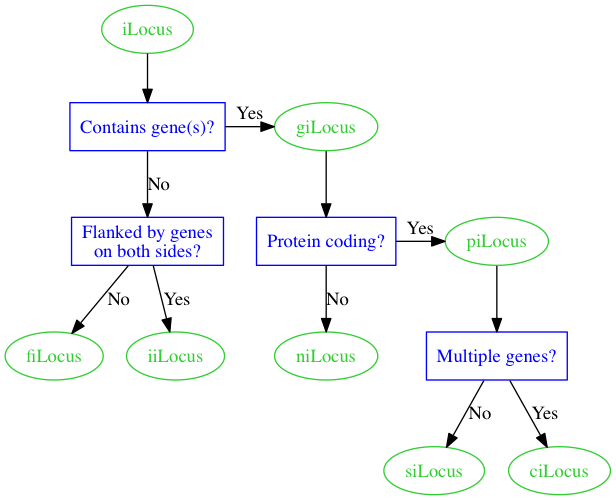
\includegraphics[width=6in]{Assets/Graphics/iLoci/ilocus-designations.png}
\centering
\caption{Designation of iLocus types shown in green, with classification logic described in blue.}
\label{Fig:iLocusDesignations}
\end{figure}

\begin{figure}[!bht]
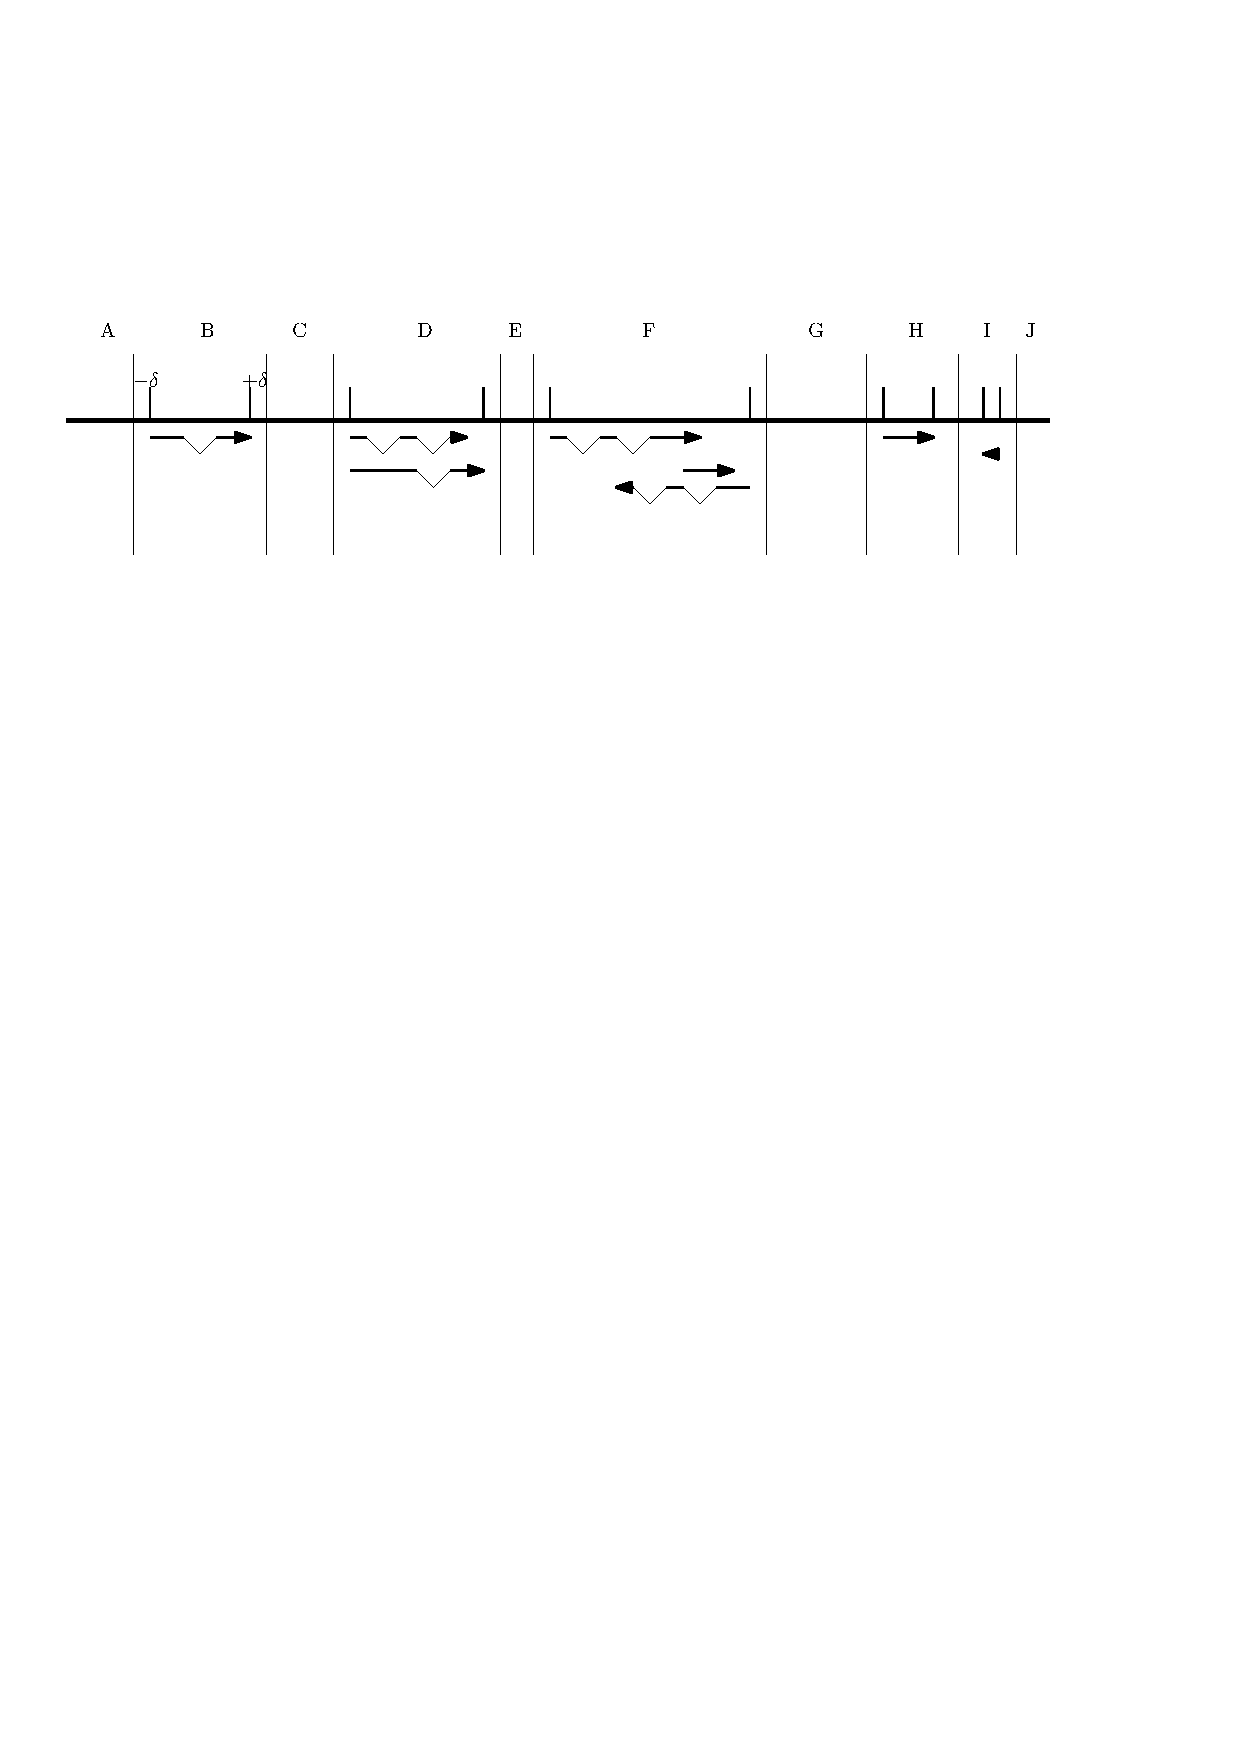
\includegraphics[width=6in]{Assets/Graphics/iLoci/ilocus-demo.pdf}
\centering
\caption{
Parsing an annotated genome sequence into iLoci.
The letters A to J indicate 10 adjacent iLoci on the genomic sequence (central horizontal line), separated by the long vertical bars.
Gene annotations are shown underneath the genome sequence.
Exons are schematized by horizontal lines, introns by the triangular thin lines below.
Arrows indicate transcriptional direction.
iLoci A, C, E, G, and J are without gene annotation, with A and J representing potentially incomplete genomic fragments (fiLoci), and C, E, and G representing intergenic regions (iiLoci).
siLoci contain a single gene annotation each and include genes with a single annotated transcript (B, H, and I) as well as genes with alternative transcripts (D).
ciLocus F contains three distinct, but overlapping genes.
The boundaries of the gene-containing iLoci (giLoci) are derived from the annotation ends, extended in each direction by $\delta$.
An exception occurs between iLoci H and I, where the extension would result in an iiLocus shorter than $\delta$: in this case, the bordering iLoci (H and I) are extended towards each other to fill the entire space.
}
\label{Fig:iLoci}
\end{figure}

\begin{figure}[!bht]
\centering
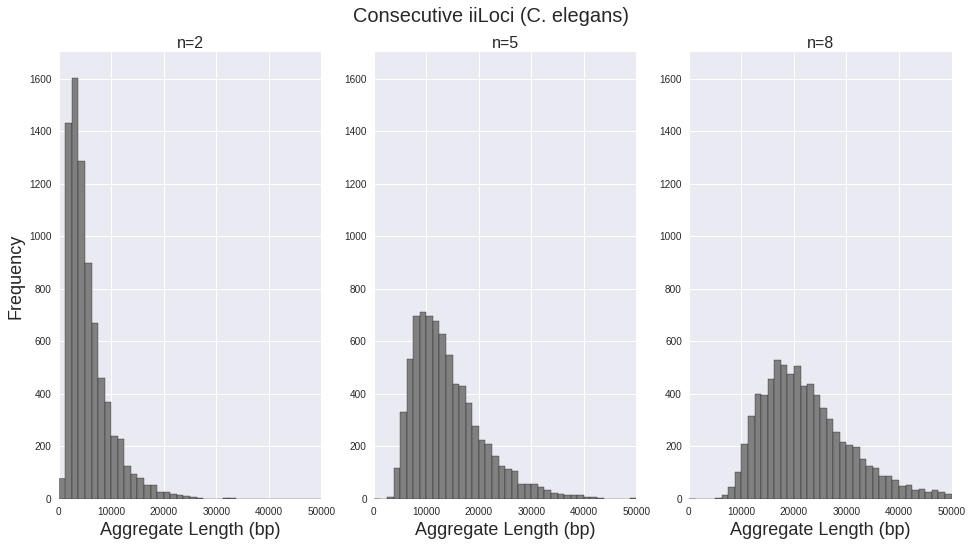
\includegraphics[width=0.65\textwidth]{Assets/Graphics/iLoci/adj-iil-cele.png}
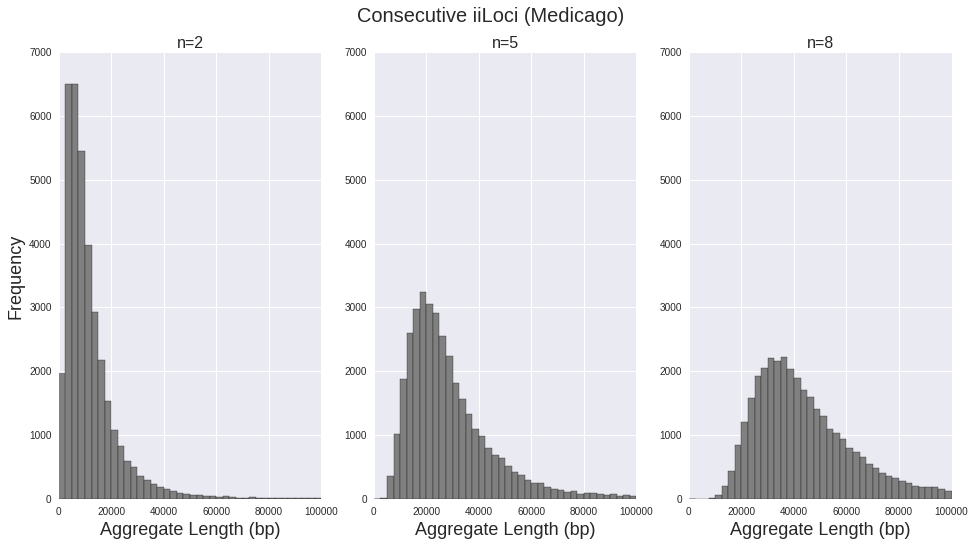
\includegraphics[width=0.65\textwidth]{Assets/Graphics/iLoci/adj-iil-mtru.png}
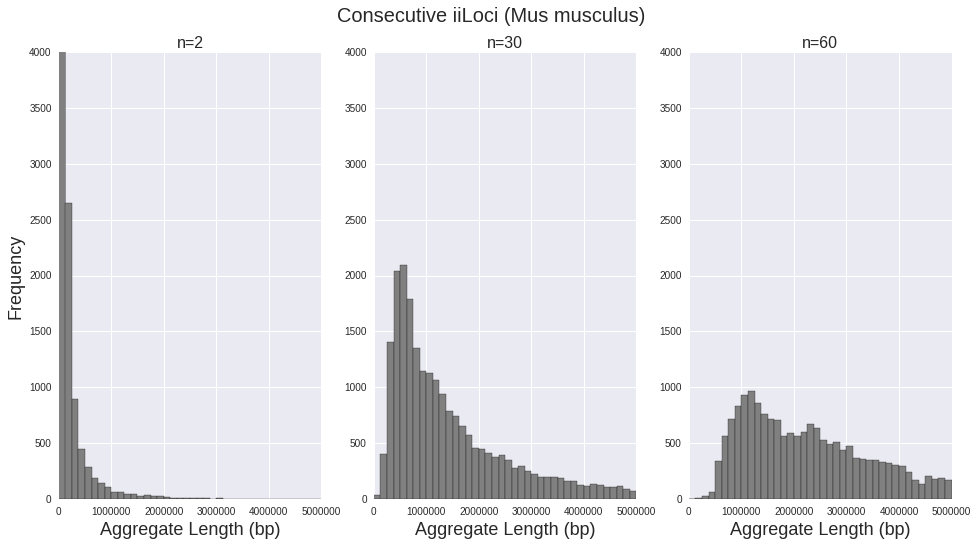
\includegraphics[width=0.65\textwidth]{Assets/Graphics/iLoci/adj-iil-mmus.png}
\caption{Aggregate lengths of $n$ adjacent iiLoci for 3 species (\textit{Caenorhabditis elegans}, \textit{Medicago truncatula}, and \textit{Mus musculus}). The value of $n$ at which the distribution of aggregate iiLocus lengths is normal is reflective of the range at which local variations in gene spacing are evened out.}
\label{Fig:AdjiiLoci}
\end{figure}

\begin{figure}[h]
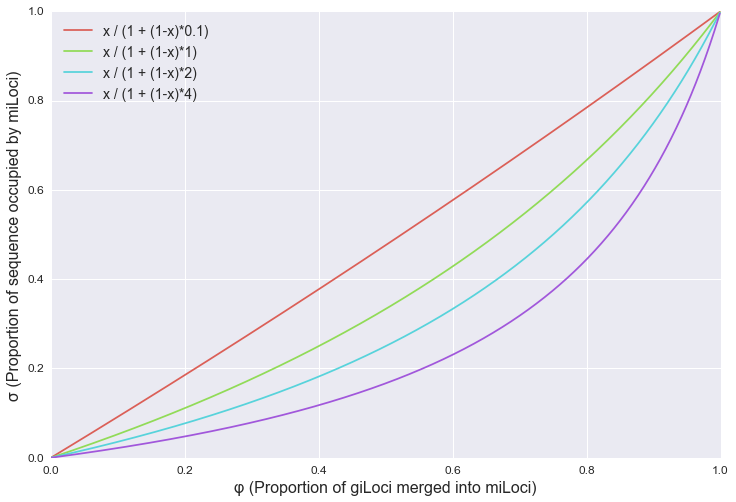
\includegraphics[width=6in]{Assets/Graphics/iLoci/compactness-theoretical.png}
\centering
\caption{Theoretical values of $\sigma$ (the proportion of genome sequence occupied by miLoci) plotted as a function of $\phi$ (the proportion of giLoci merged into miLoci) at different values of $\rho$ (the ratio of iiLocus length to giLocus length).}
\label{Fig:CompactnessModel}
\end{figure}


\begin{figure}[h]
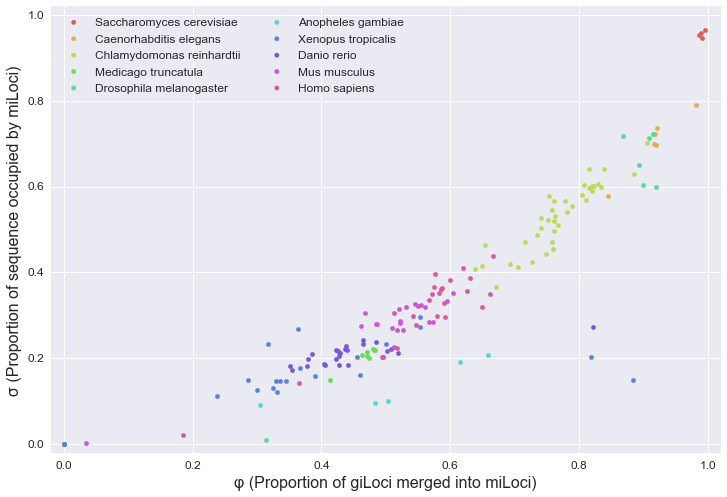
\includegraphics[width=6in]{Assets/Graphics/iLoci/modorg-compactness.png}
\centering
\caption{The genomic compactness of ten model organisms, as measured on long ($\geq$ 1 Mb) chromosome or scaffold sequences.}
\label{Fig:ModOrgCompactness}
\end{figure}

\begin{figure}[!bht]
\centering
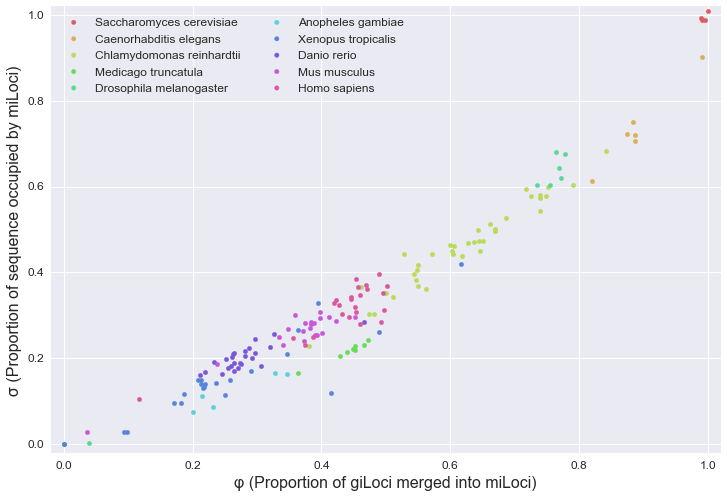
\includegraphics[width=6in]{Assets/Graphics/iLoci/compactness-shuffled.png}
\caption{Comparison of genome compactness as measured on genomic sequences as annotated (solid squares) versus the same sequences with a random arrangement of genes (hollow circles). Each point represents the average (centroid) of ($\phi, \sigma)$ values computed on all long chromosome and scaffold sequences in the corresponding assembly, as shown in \textbf{Figure \ref{Fig:ModOrgCompactness}}.}
\label{Fig:CompactnessShuffled}
\end{figure}

\clearpage

\begin{figure}[h]
\centering
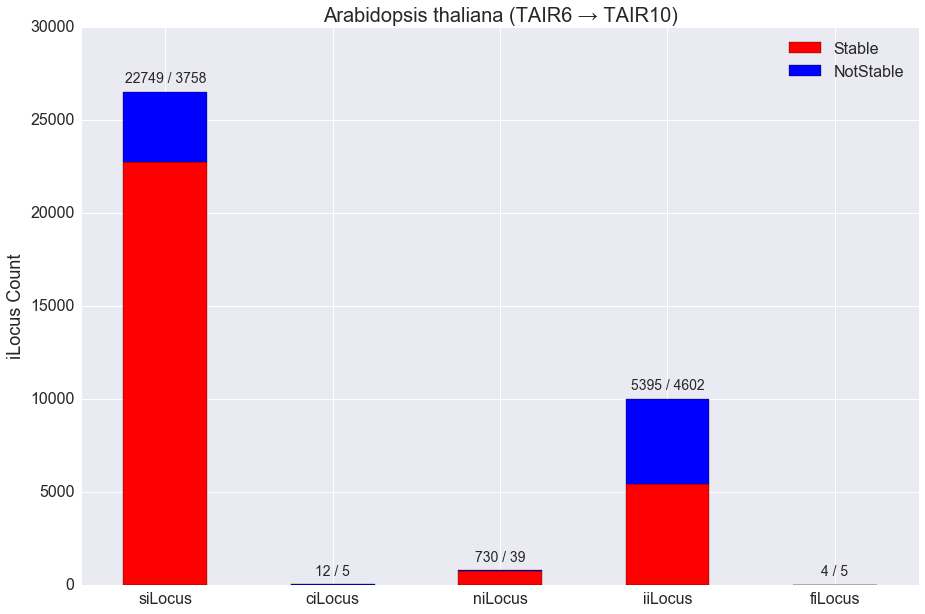
\includegraphics[width=5.5in]{Assets/Graphics/iLoci/atha-stable.png} \par
\vspace{40px}
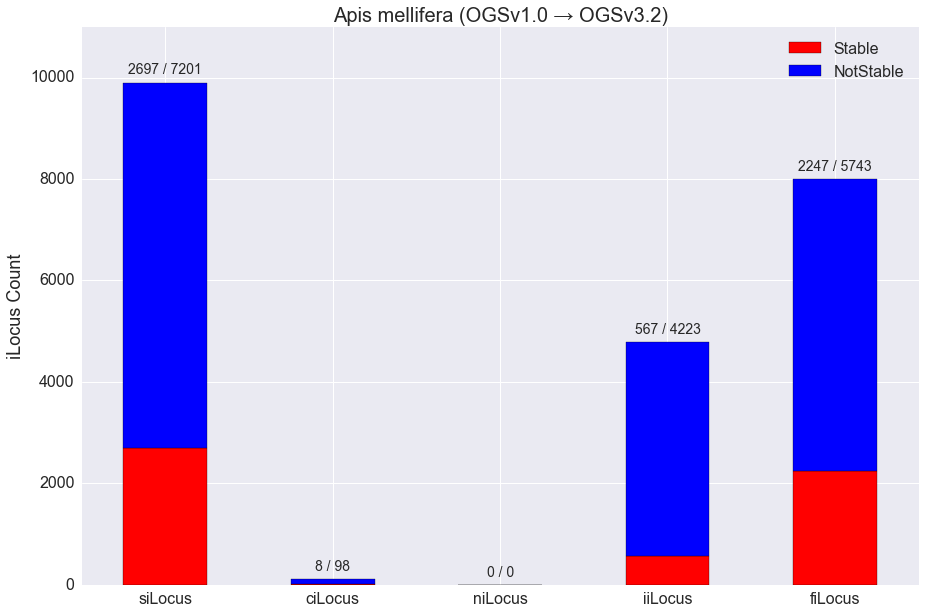
\includegraphics[width=5.5in]{Assets/Graphics/iLoci/amel-stable.png}
\caption{A breakdown of iLoci from two species by stability and classification.}
\label{Fig:iLociStable}
\end{figure}

\begin{figure}[h]
\centering
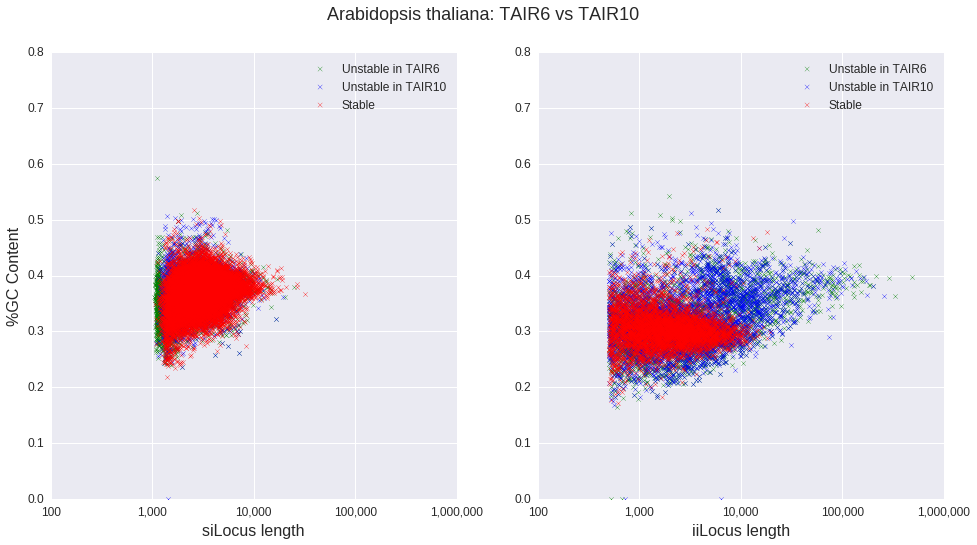
\includegraphics[width=6in]{Assets/Graphics/iLoci/atha-stable-scatter.png}
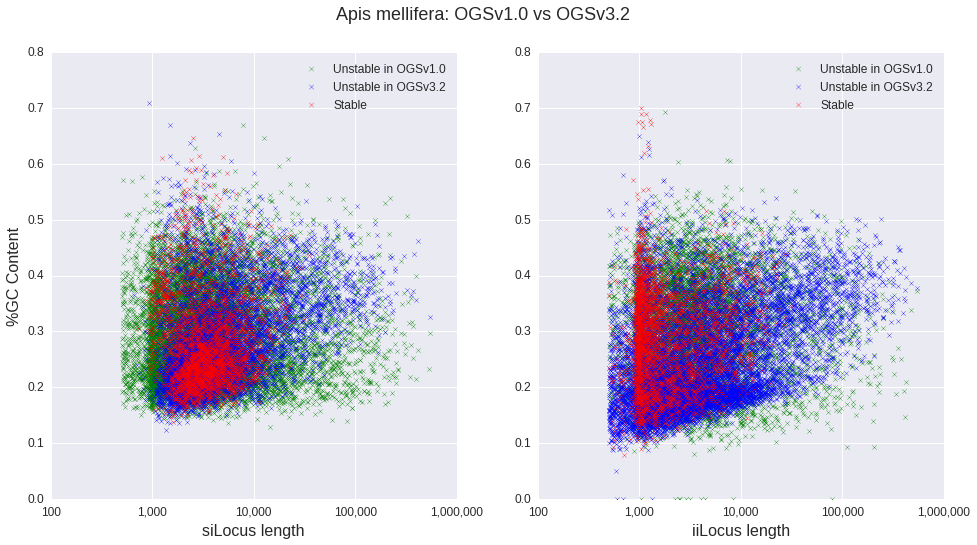
\includegraphics[width=6in]{Assets/Graphics/iLoci/amel-stable-scatter.png}
\caption{Scatter plot showing the length and nucleotide composition of iLoci from \textit{Arabidopsis thaliana} (top) and \textit{Apis mellifera} (bottom). iLoci that are stable between two assembly/annotation versions are represented by red marks, while unstable iLoci are represented by blue and green marks. siLoci are shown on the left, and iiLoci are shown on the right.}
\label{Fig:iLociStableScatter}
\end{figure}

\clearpage

\begin{figure}[h]
\centering
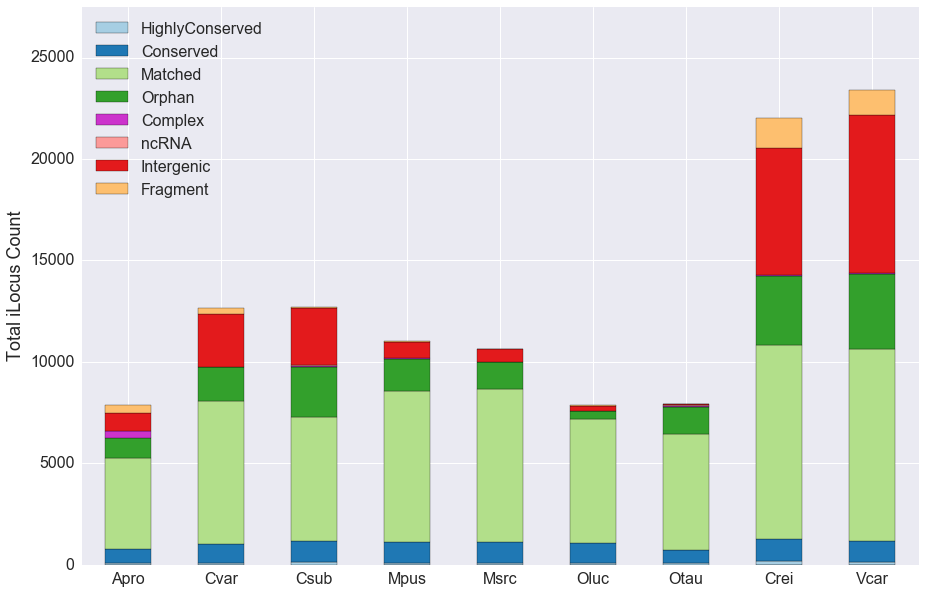
\includegraphics[width=5.5in]{Assets/Graphics/iLoci/algae-bd-counts.png} \par
\vspace{40px}
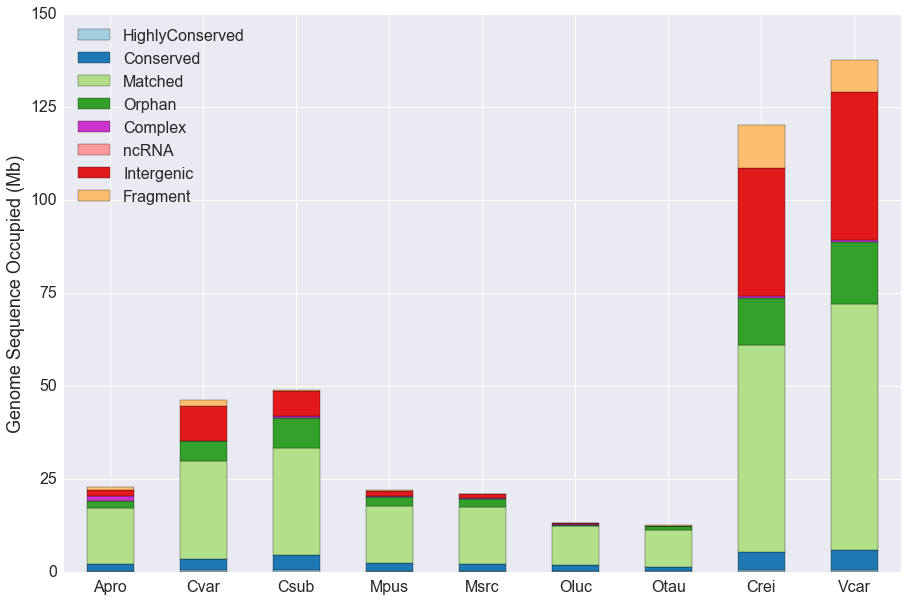
\includegraphics[width=5.5in]{Assets/Graphics/iLoci/algae-bd-bp.png}
\caption{Counts and genomic space occupied of iLoci from 9 species of green algae, categorized according to gene content and homology status.}
\label{Fig:GreenAlgaeBreakdown}
\end{figure}

\begin{figure}[h]
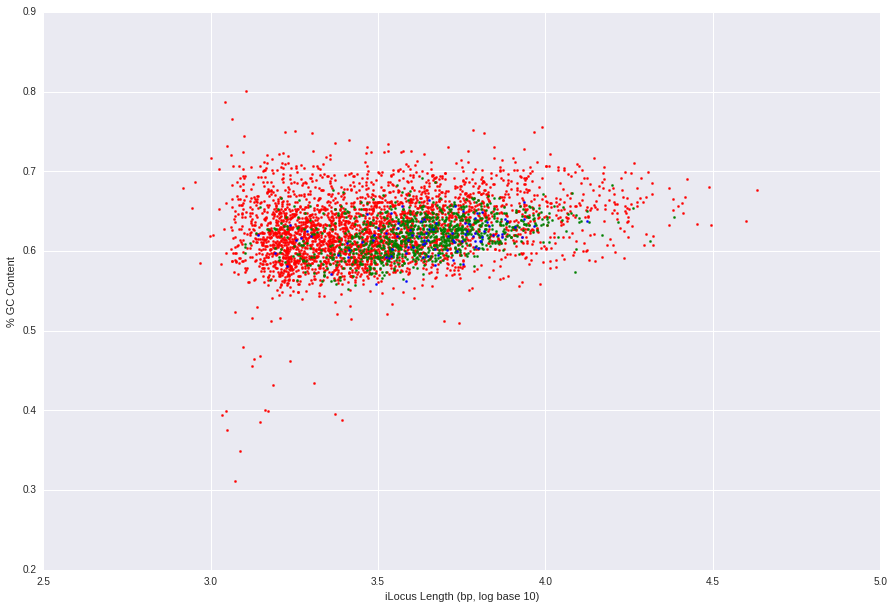
\includegraphics[width=6in]{Assets/Graphics/iLoci/crei-breakdown-scatter.png}
\centering
\caption{Plot of length and nucleotide composition for piLoci from the \textit{Chlamydomonas reinhardtii} genome. Blue point represent \textit{highly conserved piLoci}, green represent \textit{conserved piLoci}, and red represent \textit{orphan piLoci}.}
\label{Fig:CreiBreakdownScatter}
\end{figure}
